\documentclass[12pt]{article}
\usepackage{graphics,textcomp}
\newcommand{\micro}{\hbox{\textmu}}
\newcommand{\unit}[1]{\mathrm{#1}}
  \renewcommand{\deg}{\unit{deg}}
  \newcommand{\rad}{\unit{rad}}
  \newcommand{\s}{\unit{s}}
  \newcommand{\ns}{\unit{ns}}
  \newcommand{\m}{\unit{m}}
    \newcommand{\mps}{\m\,\s^{-1}}
  \newcommand{\cm}{\unit{cm}}
  \newcommand{\mm}{\unit{mm}}
  \newcommand{\mum}{\unit{\micro m}}
  \newcommand{\nm}{\unit{nm}}
  \newcommand{\kg}{\unit{kg}}
  \newcommand{\g}{\unit{g}}
  \newcommand{\Hz}{\unit{Hz}}
  \newcommand{\N}{\unit{N}}
  \newcommand{\W}{\unit{W}}
  \newcommand{\J}{\unit{J}}
  \newcommand{\V}{\unit{V}}
    \newcommand{\Vpm}{\V\,\m^{-1}}
  \newcommand{\C}{\unit{C}}
  \newcommand{\A}{\unit{A}}
  \newcommand{\ohm}{\unit{\Omega}}
  \newcommand{\F}{\unit{F}}
\newcommand{\dd}{\mathrm{d}}
\newcounter{answer}
\newenvironment{alist}{\begin{list}{(\Alph{answer})}{\usecounter{answer}}}%
  {\end{list}}
\newcommand{\explicitcorrect}[1]{[({#1})~\textbf{correct}]}
\newcommand{\correct}{~[\textbf{correct}]}
\newcommand{\source}[1]{\textsl{#1}}
\renewcommand{\emph}[1]{\textbf{#1}}
\begin{document}
\raggedright
\begin{enumerate}

\item (from lecture 2009-03-09) Two capacitors of capacitance $C_1$
  and $C_2$, with $C_1 < C_2$, are connected together in parallel.
  This makes a new device of effective capacitance $C_{\mathrm par}$.
  Then $C_1$ and $C_2$ are connected in series.  This makes a new
  device of capacitance $C_{\mathrm ser}$.  Which inequality is true?
  \begin{alist}
  \item $C_{\mathrm ser} > C_1$
  \item $C_{\mathrm ser} > C_2$
  \item $C_{\mathrm par} < C_1$
  \item $C_{\mathrm par} < C_2$
  \item $C_{\mathrm par} > C_{\mathrm ser}$\correct
  \end{alist}

\item (from lecture 2009-03-11) At which point in the diagram (below)
  is the electric field magnitude the largest?  The lines show
  equipotential surfaces, separated by constant differences in
  potential.
  \\ \resizebox{0.5\textwidth}{!}{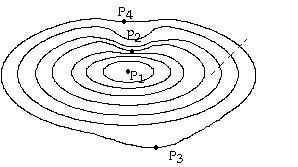
\includegraphics{30_3_1.jpg}}
  \begin{alist}
  \item $P_1$
  \item $P_2$\correct
  \item $P_3$
  \item $P_4$
  \item they are all about equal
  \end{alist}

\item (from exercise 30.28) To what potential should you charge a
  $0.5\,\micro\F$ capacitor to store $1.0\,\J$ of energy?
  \begin{alist}
  \item $1\times 10^{-3}\,\V$
  \item $2\times 10^3\,\V$\correct
  \item $4\times 10^3\,\V$
  \item $2\times 10^6\,\V$
  \item $4\times 10^6\,\V$
  \end{alist}

\item (from Chapter 30 homework) A parallel-plate capacitor is
  connected to a battery. The energy of the capacitor is $U_0$. The
  capacitor is then disconnected from the battery and the plates are
  slowly pulled apart until the plate separation is larger by a factor
  of $1.1$. The new energy of the capacitor is $U$. What is the ratio
  $U/U_0$?
  \begin{alist}
  \item $U/U_0 = \frac{1}{1.1}$
  \item $U/U_0 = 1.1$\correct
  \item $U/U_0 = \frac{1}{2}\,(1.1)^2$
  \item $U/U_0 = (1.1)^2$
  \item not enough information to say
  \end{alist}

\item (from lecture 2009-03-23) What is the approximate maximum power
  available to appliances run at $110\,\V$ on a circuit with a circuit
  breaker that trips at $15\,\A$?
  \begin{alist}
  \item $0.00067\,\W$
  \item $0.15\,\W$
  \item $6.7\,\W$
  \item $1500\,\W$\correct
  \item not within a factor of two of any of those.
  \end{alist}

\item (from lecture 2009-03-23) How many free electrons (roughly) are
  there in a cubic meter of Copper?  (Hint: In lecture we considered
  the size of an atom.)
  \begin{alist}
  \item $10^{20}$
  \item $10^{23}$
  \item $10^{26}$
  \item $10^{29}$\correct
  \item $10^{32}$
  \end{alist}

\item (from lecture 2009-03-25) Two resistors made of the same
  material have the same length $\ell$ but different cross-sectional
  areas.  Resistor $R_1$ has cross-sectional area $A$ and resistor
  $R_2$ has cross-sectional area $2\,A$.  Each resistor has the same
  voltage $V$ applied along its length.  Which statement is closest to
  true?
  \begin{alist}
  \item Resistor $R_1$ has a larger internal electric field and a larger internal current density than resistor $R_2$.
  \item Resistor $R_1$ has a smaller internal electric field and a larger internal current density than resistor $R_2$.
  \item Resistor $R_1$ has a larger internal electric field and a smaller internal current density than resistor $R_2$.
  \item Resistor $R_1$ has a smaller internal electric field and a smaller internal current density than resistor $R_2$.
  \item The two resistors have the same internal electric field and the same internal current density.\correct
  \end{alist}

\item (from conceptual question 31.13) The electric field strength
  inside a wire is doubled.  What happens?
  \begin{alist}
  \item The electron drift speed is halved and the current is halved.
  \item The electron drift speed is halved and the current is doubled.
  \item The electron drift speed is doubled and the current is halved.
  \item The electron drift speed is doubled and the current is doubled.\correct
  \item Everything is left unchanged.
  \end{alist}

\item (from Chapter 31 homework) In this junction (below) there is a
  steady-state current of $3.1\,\A$ flowing in Wire~1 in the direction
  shown, and a steady-state current of $4.2\,\A$ flowing in Wire~2 in
  the direction shown.  What is the current flowing in Wire~3?
  \\ \resizebox{0.5\textwidth}{!}{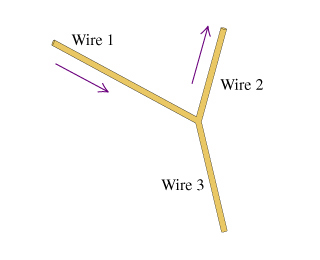
\includegraphics{1004614.jpg}}
  \begin{alist}
  \item $1.1\,\A$, towards the junction\correct
  \item $1.1\,\A$, away from the junction
  \item $7.3\,\A$, towards the junction
  \item $7.3\,\A$, away from the junction
  \item not enough information to tell
  \end{alist}

\item (from lecture 2009-03-30) Consider a spherical cell of radius
  $0.5\times10^{-6}\,\m$.  The membrane of the cell is 5\,nm thick and
  has capacitive properties no different than the electrolytic
  capacitors used in the lab.  For this cell, the resting membrane
  potential (potential difference across the cell) is 9\,mV. How many
  Potassium ions are stored on each face of the membrane? Assume all
  charges in the cell are Potassium ions.
  \begin{alist}
  \item $5\times 10^{-16}$
  \item 80
  \item 300\correct
  \item $3\times 10^{5}$
  \item $1\times 10^{29}$
  \end{alist}

\item (from lecture 2009-04-01) With the switch \emph{closed}, which
  of the identical lightbulbs that make up this circuit (below) will be
  brightest?
  \\ \resizebox{0.5\textwidth}{!}{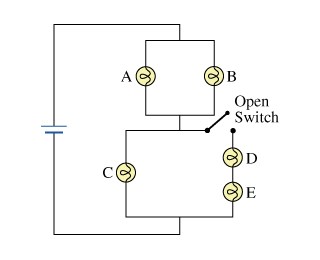
\includegraphics{15767_b.jpg}}
  \\ \explicitcorrect{C}

\item (from lecture 2009-04-01) If you multiply a capacitance by a
  resistance, what kind of quantity do you get?
  \begin{alist}
  \item a length
  \item a time\correct
  \item a current
  \item a potential difference
  \item an energy
  \end{alist}

\item (from conceptual question 32.5) Two resistors, with $R_1 < R_2$,
  are attached in parallel to a battery of voltage $V$.  Subsequently,
  they are attached in series to the same battery.  Which statment is
  true?
  \begin{alist}
  \item In parallel $R_1$ dissipates more energy; in series $R_1$ dissipates more energy
  \item In parallel $R_1$ dissipates more energy; in series $R_2$ dissipates more energy\correct
  \item In parallel $R_2$ dissipates more energy; in series $R_1$ dissipates more energy
  \item In parallel $R_2$ dissipates more energy; in series $R_2$ dissipates more energy
  \end{alist}

\item (from exercise 32.11) A household uses 860\,kWh of electricity a
  month at 110\,V.  Estimate very roughly the ``effective resistance''
  of the household.
  \begin{alist}
  \item $10\,\ohm$\correct
  \item $300\,\ohm$
  \item $10^4\,\ohm$
  \item $3\times10^5\,\ohm$
  \item $10^7\,\ohm$
  \end{alist}

\item (from Chapter 32 homework) In the circuit below, what equation
  do you get by considering Loop~1 alone?  Ignore the ammeters marked
  ``A''.
  \\ \resizebox{0.5\textwidth}{!}{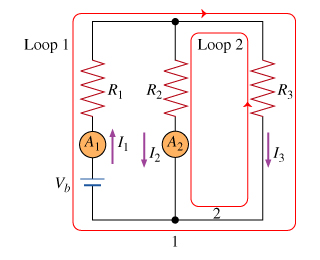
\includegraphics{36341.jpg}}
  \begin{alist}
  \item $V_b+I_1\,R_1+I_3\,R_3 = 0$
  \item $V_b+I_1\,R_1-I_3\,R_3 = 0$
  \item $V_b-I_1\,R_1+I_3\,R_3 = 0$
  \item $V_b-I_1\,R_1-I_3\,R_3 = 0$\correct
  \end{alist}

\item (from lecture 2009-04-06) The figure (below) shows a point
  charge moving in the positive $x$~direction.  A circle of radius $R$
  has been drawn around the charge with four points selected and
  labeled 1 through 4.
  \\ \resizebox{0.5\textwidth}{!}{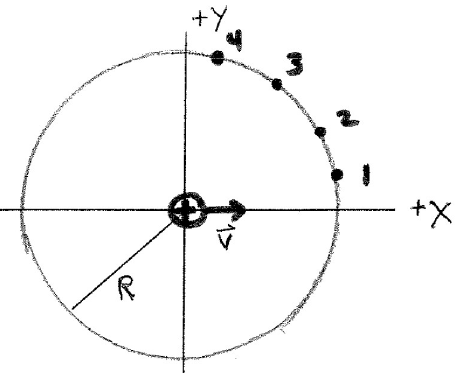
\includegraphics{andrecharge.png}} \\
  Rank the magnitudes of the magnetic field created by the moving
  charge at these four points, from largest to smallest.
  \begin{alist}
  \item $B_1 > B_2 > B_3 > B_4$
  \item $B_2 = B_3 > B_1 = B_4$
  \item $B_1 = B_2 = B_3 = B_4$
  \item $B_1 = B_4 > B_2 = B_3$
  \item $B_4 > B_3 > B_2 > B_1$\correct
  \end{alist}

\item (from lecture 2009-04-08) An electron flies in the positive
  $x$~direction alongside a long, straight wire carrying current in
  the positive $x$~direction.  The electron feels
  \begin{alist}
  \item no force at all
  \item a force towards the wire
  \item a force away from the wire\correct
  \item a force perpendicular to the velocity and perpendicular to the electron--wire separation direction
  \item a force in the positive $x$~direction
  \end{alist}

\item (from lecture 2009-04-13) Why is it useful or easy to use
  Ampere's law with a line integral along a closed loop that is
  circular and centered on a long, straight, current-carrying wire?
  \begin{alist}
  \item The magnitude of the magnetic field is constant on the loop, and the direction is tangent to the line everywhere.\correct
  \item The magnitude of the magnetic field is constant on the loop, and the direction is perpendicular to the line everywhere.
  \item The integral of the field along any closed loop is zero.
  \item There is no static electric field in the problem at all, and the magnetic field is tangent to the line everywhere.
  \item The magnetic field drops as $1/r$, and the direction of the field is perpendicular to the line everywhere.
  \end{alist}

\item (from exercise 33.37) Two 10-cm-long wires are parallel,
  side-by-side, and separated by 5\,cm.  One carries a current 5\,A.
  What current should the other carry to make the force between the
  wires exactly $5\times 10^{-6}\,\N$?
  \begin{alist}
  \item $3.9\times 10^{-12}\,\A$
  \item $0.40\,\A$
  \item $2.5\,\A$\correct
  \item $10.0\,\A$
  \item $1.0\times 10^{11}\,\A$
  \end{alist}

\item (from Chapter 33 homework) What is the direction of the net
  force on the loop from the wire in the situation depicted (below)?
  \\ \resizebox{0.5\textwidth}{!}{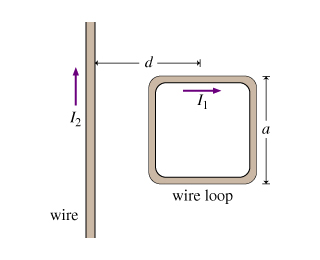
\includegraphics{20743A.jpg}}
  \begin{alist}
  \item up
  \item down
  \item left\correct
  \item right
  \end{alist}

\end{enumerate}
\end{document}
